\begin{figure}[htbp]
\centering
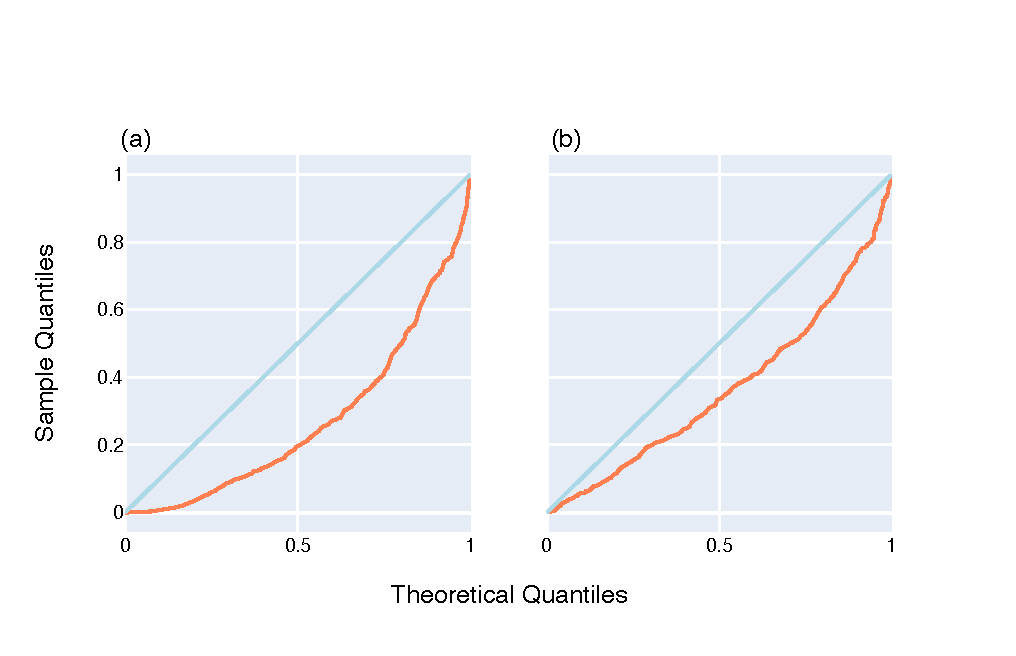
\includegraphics[width=\textwidth]{figures/plots/synthetic/lrt/197113_332182_17210-long_seq.pdf}
\caption{\textbf{Increasing the length of the alignments gives a distribution of $\hat p-$ values closer, but not consistent with theoretical expectations.} The Quantile-Quantile (Q-Q) plots compare the $\hat p$-value distribution of the test for existence in stationary simulated data to the uniform distribution. Theoretical expectation is illustrated by the diagonal. Q-Q plot for \textbf{(a)} synthetic alignments of length $300$bp, \textbf{(b)}, synthetic alignments of length $30,000$bp. Each data set contains 1,000 synthetic stationary alignments. Both data sets shown are generated from the same high JSD, high entropy seed. The other seeds exhibited the same pattern, the result is shown in the appendix Figure \ref{fig:synthetic/lrt/all-seeds}.}
\label{fig:synthetic/lrt/197113-long_seq}
\end{figure}